\documentclass[11pt]{article}

\usepackage[T1]{fontenc}
\usepackage{inconsolata}
\usepackage[default]{lato}
\usepackage{concmath}

\usepackage[a3paper, left=16mm,right=16mm, top=16mm, bottom=16mm, headheight=0pt]{geometry}
% \usepackage[fontsize=8pt]{scrextend}

\usepackage{amssymb}
\usepackage{tabularx,booktabs,multirow}

\usepackage{enumitem}
\setlist{nosep}

\usepackage{fancyvrb}

\usepackage{titlesec}
\titleformat*{\section}{\large\bfseries\scshape}
\titlespacing{\section}{0pt}{1ex}{0pt}

\usepackage{multicol}
\usepackage{tabto}
\usepackage{grid-system}

\usepackage{bytefield}
\usepackage{karnaugh-map,adjustbox}
\usepackage{tikz}
\usepackage[american]{circuitikz}
\ctikzset{
    logic ports=ieee,
    logic ports/scale=0.36
}

\setlength{\tabcolsep}{1ex}
\setlength\parindent{0pt}

\begin{document}

\pagestyle{empty}

\textbf{\Huge CS2100 Reference Sheet}

\vspace{1em}

\begin{minipage}[t]{0.68\linewidth}
	\section*{Core Instruction Set}
	\hyphenation{Unsigned}
\renewcommand{\thefootnote}{\alph{footnote}}
\newcolumntype{M}{>{\tt}l}
\newcolumntype{A}{>{\tt}l}
\newcolumntype{D}{>{\raggedright\arraybackslash\hangindent=4ex}X}

\begin{tabularx}{\textwidth}{lMAccD}
	\toprule
	\multicolumn{2}{l}{\textsc{Name}\hfill\textsc{Mnemonic}} &
	\multicolumn{2}{l}{\textsc{Operands}\hfill\textsc{Fmt}}  &
	\multicolumn{2}{l}{\textsc{Opcode/Funct}\hfill\textsc{Operation}\hfill\phantom{x}}                                                                                                      \\
	\midrule
	Add                                                      & add  & rd, rs, rt    & R & \texttt{0/0x20} & R[rd] = R[rs] + R[rt]                          \footnotemark[1]                 \\
	Add Imm.                                                 & addi & rt, rs, imm   & I & \texttt{0x08}   & R[rt] = R[rs] + SignExtImm                     \footnotemark[1]\footnotemark[2] \\
	Subtract                                                 & sub  & rd, rs, rt    & R & \texttt{0/0x22} & R[rd] = R[rs] - R[rt]                          \footnotemark[1]                 \\
	And                                                      & and  & rd, rs, rt    & R & \texttt{0/0x24} & R[rd] = R[rs] \& R[rt]                                                          \\
	And Imm.                                                 & andi & rt, rs, imm   & I & \texttt{0x0c}   & R[rt] = R[rs] \& ZeroExtImm                    \footnotemark[3]                 \\
	Or                                                       & or   & rd, rs, rt    & R & \texttt{0/0x25} & R[rd] = R[rs] | R[rt]                                                           \\
	Or Imm.                                                  & ori  & rt, rs, imm   & I & \texttt{0x0d}   & R[rt] = R[rs] | ZeroExtImm                     \footnotemark[3]                 \\
	Exclusive-Or                                             & xor  & rd, rs, rt    & R & \texttt{0/0x26} & R[rd] = R[rs] \textasciicircum{} R[rt]                                          \\
	Exclusive-Or Imm.                                        & xori & rt, rs, imm   & I & \texttt{0x0e}   & R[rt] = R[rs] \textasciicircum{} ZeroExtImm    \footnotemark[3]                 \\
	Nor                                                      & nor  & rd, rs, rt    & R & \texttt{0/0x27} & R[rd] = \textasciitilde (R[rs] | R[rt])                                         \\
	Shift Left Logical                                       & sll  & rd, rt, shamt & R & \texttt{0/0x00} & R[rd] = R[rt] <{}< shamt                                                        \\
	Shift Right Logical                                      & srl  & rd, rt, shamt & R & \texttt{0/0x02} & R[rd] = R[rt] >{}>{}> shamt                                                     \\
	Set Less Than                                            & slt  & rd, rs, rt    & R & \texttt{0/0x2a} & R[rd] = (R[rs] < R[rt]) ? 1 : 0                                                 \\
	Set Less Than Imm.                                       & slti & rt, rs, imm   & I & \texttt{0x0a}   & R[rt] = (R[rs] < SignExtImm) ? 1 : 0           \footnotemark[2]                 \\
	Load Upper Imm.                                          & lui  & rt, imm       & I & \texttt{0x0f}   & R[rt] = \{imm, 16'b0\}                                                          \\
	Load Word                                                & lw   & rt, imm(rs)   & I & \texttt{0x23}   & R[rt] = M[R[rs] + SignExtImm]                  \footnotemark[2]                 \\
	Store Word                                               & sw   & rt, imm(rs)   & I & \texttt{0x2b}   & M[R[rs] + SignExtImm] = R[rt]                  \footnotemark[2]                 \\
	Branch on Equal                                          & beq  & rs, rt, label & I & \texttt{0x04}   & if(R[rs] == R[rt]) PC = PC + 4 + BranchAddr    \footnotemark[4]                 \\
	Branch on Not Equal                                      & bne  & rs, rt, label & I & \texttt{0x05}   & if(R[rs] != R[rt]) PC = PC + 4 + BranchAddr    \footnotemark[4]                 \\
	Jump                                                     & j    & target        & J & \texttt{0x02}   & PC = JumpAddr                                  \footnotemark[5]                 \\
	Jump And Link                                            & jal  & target        & J & \texttt{0x03}   & R[31] = PC + 8; PC = JumpAddr                  \footnotemark[5]                 \\
	Jump Register                                            & jr   & rs            & R & \texttt{0/0x08} & PC = R[rs]                                                                      \\
	\bottomrule
\end{tabularx}

\end{minipage}
\hfill
\begin{minipage}[t]{0.3\linewidth}
	\section*{Register Name, Number, Use}
	\newcolumntype{U}{>{\raggedright\arraybackslash\hangindent=4ex}X}
\begin{tabularx}{\textwidth}{llU}
	\toprule
	\textsc{Name}  & \textsc{Num} & \multicolumn{1}{c}{\textsc{Use}}                      \\
	\midrule
	\verb|$zero|   & 0            & The constant value 0                                  \\
	\verb|$at|     & 1            & Assembler temporary                                   \\
	\verb|$v0-$v1| & 2 --- 3      & Values for function results and expression evaluation \\
	\verb|$a0-$a3| & 4 --- 7      & Arguments                                             \\
	\verb|$t0-$t7| & 8 --- 15     & Temporaries                                           \\
	\verb|$s0-$s7| & 16 --- 23    & Saved temporaries                                     \\
	\verb|$t8-$t9| & 24 --- 25    & Temporaries                                           \\
	\verb|$k0-$k1| & 26 --- 27    & Reserved for os kernel                                \\
	\verb|$gp|     & 28           & Global pointer                                        \\
	\verb|$sp|     & 29           & Stack pointer                                         \\
	\verb|$fp|     & 30           & Frame pointer                                         \\
	\verb|$ra|     & 31           & Return address                                        \\
	\bottomrule
\end{tabularx}


	\begin{enumerate}[label=\alph*.,leftmargin=1em]
	\item {May cause overflow exception}
	\item {SignExtImm = \{16\{imm[15]\}, imm\}}
	\item {ZeroExtImm = \{16\{1b'0\}, imm\}}
	\item {BranchAddr = \{14\{imm[15]\}, imm, 2'b0\}}
	\item {JumpAddr = \{PC+4[31:28], addr, 2'b0\}}
	\item {Operands considered unsigned numbers \\ (vs. 2's comp.)}
\end{enumerate}

\end{minipage}



\vfill

\begin{minipage}[t]{0.64\linewidth}
	\section*{MIPS Data Path with Control Unit}
	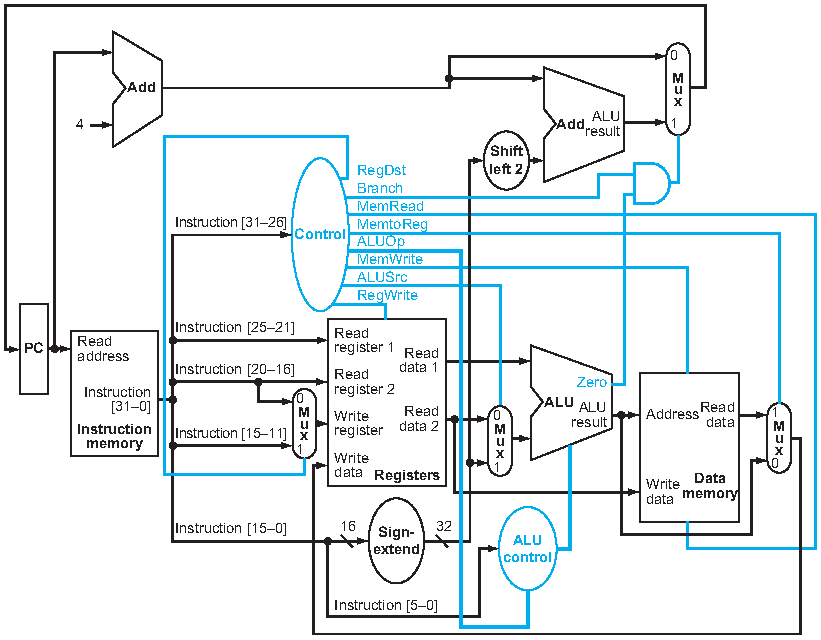
\includegraphics[width=\linewidth]{mips-cpu/fig417.pdf}

	\section*{MIPS Control Signals}
	% \begin{tabular}[t]{ccccc}
% 	\toprule
% 	         & R-type & LW   & SW   & BEQ  \\
% 	\midrule
% 	RegDst   & {1}    & {0}  & {x}  & {x}  \\
% 	ALUSrc   & {0}    & {1}  & {1}  & {0}  \\
% 	MemToReg & {0}    & {1}  & {x}  & {x}  \\
% 	RegWrite & {1}    & {1}  & {0}  & {0}  \\
% 	MemRead  & {0}    & {1}  & {0}  & {0}  \\
% 	MemWrite & {0}    & {0}  & {1}  & {0}  \\
% 	Branch   & {0}    & {0}  & {0}  & {1}  \\
% 	ALUop    & {10}   & {00} & {00} & {01} \\
% 	\bottomrule
% \end{tabular}
\begin{tabular}[t]{ccccccccc}
	\toprule
	         & RegDst & ALUSrc & MemToReg & RegWrite & MemRead & MemWrite & Branch & ALUOp \\
	\midrule
	R-format & 1      & 0      & 0        & 1        & 0       & 0        & 0      & 10    \\
	lw       & 0      & 1      & 1        & 1        & 1       & 0        & 0      & 00    \\
	sw       & x      & 1      & x        & 0        & 0       & 1        & 0      & 00    \\
	beq      & x      & 0      & x        & 0        & 0       & 0        & 1      & 01    \\
	\bottomrule
\end{tabular}

\end{minipage}
\hfill
\begin{minipage}[t]{0.35\linewidth}
	\section*{Basic Instruction Formats}
	\vspace{1em}
	\begin{itemize}[leftmargin=1em]
	\setlength\itemsep{1em}
	\item[R]
	      \begin{bytefield}[boxformatting=\centering\small,bitwidth=0.03125\linewidth,bitheight=1.5em]{32}
		      \bitheader[endianness=big]{0,5,6,10,11,15,16,20,21,25,26,31} \\
		      \bitbox{6}{opcode} &
		      \bitbox{5}{rs} &
		      \bitbox{5}{rt} &
		      \bitbox{5}{rd} &
		      \bitbox{5}{shamt} &
		      \bitbox{6}{funct}
	      \end{bytefield}
	\item[I]
	      \begin{bytefield}[boxformatting=\centering\small,bitwidth=0.03125\linewidth,bitheight=1.5em]{32}
		      \bitheader[endianness=big]{0,15,16,20,21,25,26,31} \\
		      \bitbox{6}{opcode} &
		      \bitbox{5}{rs} &
		      \bitbox{5}{rt} &
		      \bitbox{16}{immediate}
	      \end{bytefield}
	\item[J]
	      \begin{bytefield}[boxformatting=\centering\small,bitwidth=0.03125\linewidth,bitheight=1.5em]{32}
		      \bitheader[endianness=big]{0,25,26,31} \\
		      \bitbox{6}{opcode} &
		      \bitbox{26}{address}
	      \end{bytefield}
\end{itemize}


	\vspace{2ex}

	\section*{1-bit ALU}

	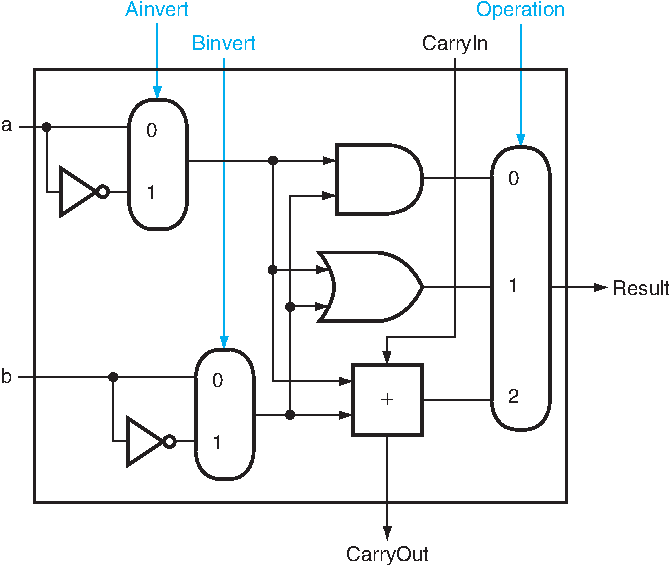
\includegraphics[width=\linewidth]{mips-cpu/alu.pdf}

	\vspace{1ex}
	\vspace{0.5mm}
	\begin{tabular}[t]{c|ccc|c}
	\toprule
	ALUControl & Ainvert & Binvert & Operation & Action \\
	\midrule
	{0000}     & 0       & 0       & 00        & and    \\
	{0001}     & 0       & 0       & 01        & or     \\
	{0010}     & 0       & 0       & 10        & add    \\
	{0110}     & 0       & 1       & 10        & sub    \\
	{0111}     & 0       & 1       & 11        & slt    \\
	{1100}     & 1       & 1       & 00        & nor    \\
	\bottomrule
\end{tabular}

\end{minipage}



\vfill

\begin{minipage}[t]{\linewidth}
	\begin{minipage}[t]{0.5\textwidth}
		\section*{MIPS ALUControl}
		\begin{tabular}[t]{llcclc}
	\toprule
	\multicolumn{1}{c}{Instruction} &
	\multicolumn{1}{c}{Opcode}      &
	ALUOp                           &
	Funct                           &
	\multicolumn{1}{c}{ALU Action}  &
	\multicolumn{1}{c}{ALUControl}                                                               \\
	\midrule
	\texttt{lw}                     & LW           & {00} & {xxxxxx} & add              & {0010} \\
	\texttt{sw}                     & SW           & {00} & {xxxxxx} & add              & {0010} \\
	\texttt{beq}                    & Branch equal & {01} & {xxxxxx} & subtract         & {0110} \\
	\texttt{add}                    & R-type       & {10} & {100000} & add              & {0010} \\
	\texttt{sub}                    & R-type       & {10} & {100010} & subtract         & {0110} \\
	\texttt{and}                    & R-type       & {10} & {100100} & and              & {0000} \\
	\texttt{or}                     & R-type       & {10} & {100101} & or               & {0001} \\
	\texttt{slt}                    & R-type       & {10} & {101010} & set on less than & {0111} \\
	\bottomrule
\end{tabular}

	\end{minipage}
	\begin{minipage}[t]{0.28\textwidth}
	\end{minipage}
\end{minipage}

\vfill

\clearpage

\begin{minipage}[t]{0.68\linewidth}
	\begin{minipage}[t]{0.48\linewidth}
		\section*{4-bit Number Systems}
		\begin{tabular}{cccc}
	\toprule
	Value & Sign \& Mag & 1s Comp. & 2s Comp. \\
	\midrule
	+7    & {0111}      & {0111}   & {0111}   \\
	+6    & {0110}      & {0110}   & {0110}   \\
	+5    & {0101}      & {0101}   & {0101}   \\
	+4    & {0100}      & {0100}   & {0100}   \\
	+3    & {0011}      & {0011}   & {0011}   \\
	+2    & {0010}      & {0010}   & {0010}   \\
	+1    & {0001}      & {0001}   & {0001}   \\
	+0    & {0000}      & {0000}   & {0000}   \\
	\midrule
	-0    & {1000}      & {1111}   & {-}      \\
	-1    & {1001}      & {1110}   & {1111}   \\
	-2    & {1010}      & {1101}   & {1110}   \\
	-3    & {1011}      & {1100}   & {1101}   \\
	-4    & {1100}      & {1011}   & {1100}   \\
	-5    & {1101}      & {1010}   & {1011}   \\
	-6    & {1110}      & {1001}   & {1010}   \\
	-7    & {1111}      & {1000}   & {1001}   \\
	-8    & {-}         & {-}      & {1000}   \\
	\bottomrule
\end{tabular}

	\end{minipage}
    \hfill
    \begin{minipage}[t]{0.48\linewidth}
		\section*{Nibble}
		\begin{tabular}{ccccc}
	\toprule
	HEX & DEC & BIN    & 1s Comp. & 2s Comp. \\
	\midrule
	{0} & 0   & {0000} & +0       & +0       \\
	{1} & 1   & {0001} & +1       & +1       \\
	{2} & 2   & {0010} & +2       & +2       \\
	{3} & 3   & {0011} & +3       & +3       \\
	{4} & 4   & {0100} & +4       & +4       \\
	{5} & 5   & {0101} & +5       & +5       \\
	{6} & 6   & {0110} & +6       & +6       \\
	{7} & 7   & {0111} & +7       & +7       \\
	{8} & 8   & {1000} & -7       & -8       \\
	{9} & 9   & {1001} & -6       & -7       \\
	{A} & 10  & {1010} & -5       & -6       \\
	{B} & 11  & {1011} & -4       & -5       \\
	{C} & 12  & {1100} & -3       & -4       \\
	{D} & 13  & {1101} & -2       & -3       \\
	{E} & 14  & {1110} & -1       & -2       \\
	{F} & 15  & {1111} & -0       & -1       \\
	\bottomrule
\end{tabular}

	\end{minipage}

	\vspace{1em}

	\begin{minipage}[t]{0.64\linewidth}
		\section*{IEEE 754 Floating Point Standard}
$$
    (-1)^S \times M \times 2^{E-B}
$$

Single Precision Format (Bias = 127) \vspace{1em}
\begin{center}
    \begin{bytefield}[boxformatting=\centering\small,bitwidth=0.03\linewidth,bitheight=1.5em]{32}
        \bitheader[endianness=big]{0,22,23,30,31} \\
        \bitbox{1}{S} &
        \bitbox{8}{Exponent} &
        \bitbox{23}{Mantissa}
    \end{bytefield}
\end{center}

Double Precision Format (Bias = 1023)
\begin{center}
    \begin{bytefield}[boxformatting=\centering\small,bitwidth=0.03\linewidth,bitheight=1.5em]{32}
        \bitheader[lsb=32,endianness=big]{32,51,52,62,63} \\
        \bitbox{1}{S} &
        \bitbox{11}{Exponent} &
        \bitbox{20}{Mantissa[51:32]} \\
        \bitheader[endianness=big]{0,31} \\
        \bitbox{32}{Mantissa[31:0]}
    \end{bytefield}
\end{center}

	\end{minipage}
	\hfill
	\begin{minipage}[t]{0.32\linewidth}
		\section*{K-Map}

\begin{center}
\begin{karnaugh-map}(label=corner)[4][4][1][$D$][$C$][$B$][$A$]
\manualterms{$m_0$, $m_{1}$, $m_{2}$, $m_{3}$, $m_{4}$, $m_{5}$, $m_{6}$, $m_{7}$, $m_{8}$, $m_{9}$, $m_{10}$, $m_{11}$, $m_{12}$, $m_{13}$, $m_{14}$, $m_{15}$}
\end{karnaugh-map}
\end{center}

	\end{minipage}

	\begin{minipage}[t]{\linewidth}
		\section*{Laws of Boolean Algebra}
\begin{tabular}{lll}
    \toprule
    \textbf{Name}     & \textbf{AND}                                                  & \textbf{OR}                                                     \\
    \midrule
    Identity Laws     & $x \cdot 1 = x$                                               & $x + 0 = x$                                                     \\
    Complement Laws   & $x \cdot x' = 0$                                              & $x + x' = 1$                                                    \\
    Commutative Laws  & $x \cdot y = y \cdot x$                                       & $x + y = y + x$                                                 \\
    Associative Laws  & $x \cdot (y \cdot z) = (x \cdot y) \cdot z$                   & $x + (y + z) = (x + y) + z$                                     \\
    Distributive Laws & $x \cdot (y + z) = x \cdot y + x \cdot z$                     & $x + y \cdot z = (x + y) \cdot (x + z)$                         \\
    \midrule
    Idempotency       & $x \cdot x = x$                                               & $x + x = x$                                                     \\
    Zero/One Element  & $x \cdot 0 = 0$                                               & $x + 1 = 1$                                                     \\
    Involution        & $(x')' = x$                                                   &                                                                 \\
    Absorption 1      & $x + x \cdot y = x$                                           & $x \cdot (x + y) = x$                                           \\
    Absorption 2      & $x + x' \cdot y = x + y$                                      & $x \cdot (x' + y) = x \cdot y$                                  \\
    DeMorgan's Law    & $(x \cdot y)' = x' + y'$                                      & $(x + y)' = x' \cdot y'$                                        \\
    Consensus         & $x \cdot y + x' \cdot z + y \cdot z = x \cdot y + x' \cdot z$ & $(x + y) \cdot (x' + z) \cdot (y + z) = (x + y) \cdot (x' + z)$ \\
    \bottomrule
\end{tabular}

	\end{minipage}

	\vspace{1em}

	\begin{minipage}[t]{\linewidth}
		% chktex-file 44
\section*{Truth Tables}

\vspace{1ex}

\begin{Row}
	\begin{Cell}{1}
		{AND}\vspace{0.5ex}

		\centering
		\begin{circuitikz}[]
			\draw (0,0) 	node[scale=2,and port](G){};
			\draw (G.in 1) 	node[anchor=east]{$a$};
			\draw (G.in 2) 	node[anchor=east]{$b$};
			\draw (G.out) 	node[anchor=west]{$a \cdot b$};
		\end{circuitikz}
	\end{Cell}
	\begin{Cell}{1}
		{OR}\vspace{0.5ex}

		\centering
		\begin{circuitikz}[]
			\draw (0,0) 	node[scale=2,or port](G){};
			\draw (G.in 1) 	node[anchor=east]{$a$};
			\draw (G.in 2) 	node[anchor=east]{$b$};
			\draw (G.out) 	node[anchor=west]{$a + b$};
		\end{circuitikz}
	\end{Cell}
	\begin{Cell}{1}
		{XOR}\vspace{0.5ex}

		\centering
		\begin{circuitikz}[]
			\draw (0,0) 	node[scale=2,xor port](G){};
			\draw (G.in 1) 	node[anchor=east]{$a$};
			\draw (G.in 2) 	node[anchor=east]{$b$};
			\draw (G.out) 	node[anchor=west]{$a \oplus b$};
		\end{circuitikz}
	\end{Cell}
	\begin{Cell}{1}
		{NOT}\vspace{0.5ex}

		\centering
		\begin{circuitikz}[]
			\draw (0,0) 	node[scale=2,not port](G){};
			\draw (G.in) 	node[anchor=east]{$a$};
			\draw (G.out) 	node[anchor=west]{$\overline{a}$};
		\end{circuitikz}
	\end{Cell}
\end{Row}

\vspace{1em}

\begin{Row}
	\begin{Cell}{1}
		\centering
		\begin{tabular}{cc|c}
			\toprule
			$a$ & $b$ & $a\cdot b$ \\
			\midrule
			$0$ & $0$ & $0$        \\
			$0$ & $1$ & $0$        \\
			$1$ & $0$ & $0$        \\
			$1$ & $1$ & $1$        \\
			\bottomrule
		\end{tabular}
	\end{Cell}
	\begin{Cell}{1}
		\centering
		\begin{tabular}{cc|c}
			\toprule
			$a$ & $b$ & $a+b$ \\
			\midrule
			$0$ & $0$ & $0$   \\
			$0$ & $1$ & $1$   \\
			$1$ & $0$ & $1$   \\
			$1$ & $1$ & $1$   \\
			\bottomrule
		\end{tabular}
	\end{Cell}
	\begin{Cell}{1}
		\centering
		\begin{tabular}{cc|c}
			\toprule
			$a$ & $b$ & $a \oplus b$ \\
			\midrule
			$0$ & $0$ & $0$          \\
			$0$ & $1$ & $1$          \\
			$1$ & $0$ & $1$          \\
			$1$ & $1$ & $0$          \\
			\bottomrule
		\end{tabular}
	\end{Cell}
	\begin{Cell}{1}
		\centering
		\begin{tabular}{c|c}
			\toprule
			$a$ & $\overline{a}$ \\
			\midrule
			$0$ & $1$            \\
			$1$ & $0$            \\
			\bottomrule
		\end{tabular}
	\end{Cell}
\end{Row}

\vspace{1em}

\begin{Row}
	\begin{Cell}{1}
		{NAND}\vspace{0.5ex}

		\centering
		\begin{circuitikz}[]
			\draw (0,0) 	node[scale=2,nand port](G){};
			\draw (G.in 1) 	node[anchor=east]{$a$};
			\draw (G.in 2) 	node[anchor=east]{$b$};
			\draw (G.out) 	node[anchor=west]{$\overline{a \cdot b}$};
		\end{circuitikz}
	\end{Cell}
	\begin{Cell}{1}
		{NOR}\vspace{0.5ex}

		\centering
		\begin{circuitikz}[]
			\draw (0,0) 	node[scale=2,nor port](G){};
			\draw (G.in 1) 	node[anchor=east]{$a$};
			\draw (G.in 2) 	node[anchor=east]{$b$};
			\draw (G.out) 	node[anchor=west]{$\overline{a + b}$};
		\end{circuitikz}
	\end{Cell}
	\begin{Cell}{1}
		{XNOR}\vspace{0.5ex}

		\centering
		\begin{circuitikz}[]
			\draw (0,0) 	node[scale=2,xnor port](G){};
			\draw (G.in 1) 	node[anchor=east]{$a$};
			\draw (G.in 2) 	node[anchor=east]{$b$};
			\draw (G.out) 	node[anchor=west]{$\overline{a \oplus b}$};
		\end{circuitikz}
	\end{Cell}
	\begin{Cell}{1}
		\phantom{x}
	\end{Cell}
\end{Row}

\vspace{1ex}

\begin{Row}
	\begin{Cell}{1}
		\centering
		\begin{tabular}{cc|c}
			\toprule
			$a$ & $b$ & $\overline{a\cdot b}$ \\
			\midrule
			$0$ & $0$ & $1$                   \\
			$0$ & $1$ & $1$                   \\
			$1$ & $0$ & $1$                   \\
			$1$ & $1$ & $0$                   \\
			\bottomrule
		\end{tabular}
	\end{Cell}
	\begin{Cell}{1}
		\centering
		\begin{tabular}{cc|c}
			\toprule
			$a$ & $b$ & $\overline{a+b}$ \\
			\midrule
			$0$ & $0$ & $1$              \\
			$0$ & $1$ & $0$              \\
			$1$ & $0$ & $0$              \\
			$1$ & $1$ & $0$              \\
			\bottomrule
		\end{tabular}
	\end{Cell}
	\begin{Cell}{1}
		\centering
		\begin{tabular}{cc|c}
			\toprule
			$a$ & $b$ & $\overline{a \oplus b}$ \\
			\midrule
			$0$ & $0$ & $1$                     \\
			$0$ & $1$ & $0$                     \\
			$1$ & $0$ & $0$                     \\
			$1$ & $1$ & $1$                     \\
			\bottomrule
		\end{tabular}
	\end{Cell}
	\begin{Cell}{1}
		\phantom{x}
	\end{Cell}
\end{Row}

	\end{minipage}
\end{minipage}
\hfill
\begin{minipage}[t]{0.28\linewidth}
	\section*{ASCII}
    \centering
	
\newcolumntype{C}{>{\ttfamily}c}
\newcolumntype{R}{>{\ttfamily}r}
\begin{tabular}{C|RRC|RRC}
	\toprule
	BIN    & DEC & HEX & ASCII & DEC & HEX & ASCII            \\
	\midrule
	000000 & 0   & 0   & NUL   & 64  & 40  & @                \\
	000001 & 1   & 1   & SOH   & 65  & 41  & A                \\
	000010 & 2   & 2   & STX   & 66  & 42  & B                \\
	000011 & 3   & 3   & ETX   & 67  & 43  & C                \\
	000100 & 4   & 4   & EOT   & 68  & 44  & D                \\
	000101 & 5   & 5   & ENQ   & 69  & 45  & E                \\
	000110 & 6   & 6   & ACK   & 70  & 46  & F                \\
	000111 & 7   & 7   & BEL   & 71  & 47  & G                \\
	001000 & 8   & 8   & BS    & 72  & 48  & H                \\
	001001 & 9   & 9   & HT    & 73  & 49  & I                \\
	001010 & 10  & a   & LF    & 74  & 4a  & J                \\
	001011 & 11  & b   & VT    & 75  & 4b  & K                \\
	001100 & 12  & c   & FF    & 76  & 4c  & L                \\
	001101 & 13  & d   & CR    & 77  & 4d  & M                \\
	001110 & 14  & e   & SO    & 78  & 4e  & N                \\
	001111 & 15  & f   & SI    & 79  & 4f  & O                \\
	010000 & 16  & 10  & DLE   & 80  & 50  & P                \\
	010001 & 17  & 11  & DC1   & 81  & 51  & Q                \\
	010010 & 18  & 12  & DC2   & 82  & 52  & R                \\
	010011 & 19  & 13  & DC3   & 83  & 53  & S                \\
	010100 & 20  & 14  & DC4   & 84  & 54  & T                \\
	010101 & 21  & 15  & NAK   & 85  & 55  & U                \\
	010110 & 22  & 16  & SYN   & 86  & 56  & V                \\
	010111 & 23  & 17  & ETB   & 87  & 57  & W                \\
	011000 & 24  & 18  & CAN   & 88  & 58  & X                \\
	011001 & 25  & 19  & EM    & 89  & 59  & Y                \\
	011010 & 26  & 1a  & SUB   & 90  & 5a  & Z                \\
	011011 & 27  & 1b  & ESC   & 91  & 5b  & [                \\
	011100 & 28  & 1c  & FS    & 92  & 5c  & \textbackslash   \\
	011101 & 29  & 1d  & GS    & 93  & 5d  & ]                \\
	011110 & 30  & 1e  & RS    & 94  & 5e  & \textasciicircum \\
	011111 & 31  & 1f  & US    & 95  & 5f  & \textunderscore  \\
	100000 & 32  & 20  & Space & 96  & 60  & `                \\
	100001 & 33  & 21  & !     & 97  & 61  & a                \\
	100010 & 34  & 22  & "     & 98  & 62  & b                \\
	100011 & 35  & 23  & \#    & 99  & 63  & c                \\
	100100 & 36  & 24  & \$    & 100 & 64  & d                \\
	100101 & 37  & 25  & \%    & 101 & 65  & e                \\
	100110 & 38  & 26  & \&    & 102 & 66  & f                \\
	100111 & 39  & 27  & '     & 103 & 67  & g                \\
	101000 & 40  & 28  & (     & 104 & 68  & h                \\
	101001 & 41  & 29  & )     & 105 & 69  & i                \\
	101010 & 42  & 2a  & *     & 106 & 6a  & j                \\
	101011 & 43  & 2b  & +     & 107 & 6b  & k                \\
	101100 & 44  & 2c  & ,     & 108 & 6c  & l                \\
	101101 & 45  & 2d  & -     & 109 & 6d  & m                \\
	101110 & 46  & 2e  & .     & 110 & 6e  & n                \\
	101111 & 47  & 2f  & /     & 111 & 6f  & o                \\
	110000 & 48  & 30  & 0     & 112 & 70  & p                \\
	110001 & 49  & 31  & 1     & 113 & 71  & q                \\
	110010 & 50  & 32  & 2     & 114 & 72  & r                \\
	110011 & 51  & 33  & 3     & 115 & 73  & s                \\
	110100 & 52  & 34  & 4     & 116 & 74  & t                \\
	110101 & 53  & 35  & 5     & 117 & 75  & u                \\
	110110 & 54  & 36  & 6     & 118 & 76  & v                \\
	110111 & 55  & 37  & 7     & 119 & 77  & w                \\
	111000 & 56  & 38  & 8     & 120 & 78  & x                \\
	111001 & 57  & 39  & 9     & 121 & 79  & y                \\
	111010 & 58  & 3a  & :     & 122 & 7a  & z                \\
	111011 & 59  & 3b  & ;     & 123 & 7b  & \{               \\
	111100 & 60  & 3c  & <     & 124 & 7c  & |                \\
	111101 & 61  & 3d  & =     & 125 & 7d  & \}               \\
	111110 & 62  & 3e  & >     & 126 & 7e  & \textasciitilde  \\
	111111 & 63  & 3f  & ?     & 127 & 7f  & DEL              \\
	\bottomrule
\end{tabular}

\end{minipage}

\end{document}
